\subsection{m6a Family}
The m6a host features the AMD EPYC 7R13 Processor. Table \ref{tab::max_m6a} captures the maximum 
achievable performance degradation on the test node while adding busy or idle neighbors. 

\begin{table}[H]
\begin{center}
\begin{tabular}{ |c|c|c|c|c|c }
 Instance type & large & xlarge & 2xlarge & 4xlarge \\
 \hline
 Maximum Nodes & 96 & 48 & 24 & 12  \\
 \hline
Degradation (Busy) \% & 10 & 9.5 & 11.1 & 11.4  \\ 
\hline 
Degradation (Idle) \% & 0.05 & 0.06 & 0.06 & 0.05  \\ 
\end{tabular}
\end{center}
\caption{Maximum achievable performance degradation on our test node across various m6i instance types}
\label{tab::max_m6a}
\end{table}
\noindent
When adding busy neighbors, we notice close percentages of performance 
degradation across the different instance types,  with an average of 10\%. 
When alone on the dedicated host, the test node started from roughly the same initial nominal value 
across all the instance types (7.09 seconds). 
Figure \ref{fig::m6a_metal_vs_VMs} compares the runtime on our 
test node when adding busy m6a.4xlarge neighbors to the runtime of running the threads natively on 
the m6a.metal instance. 

\begin{figure}[H]
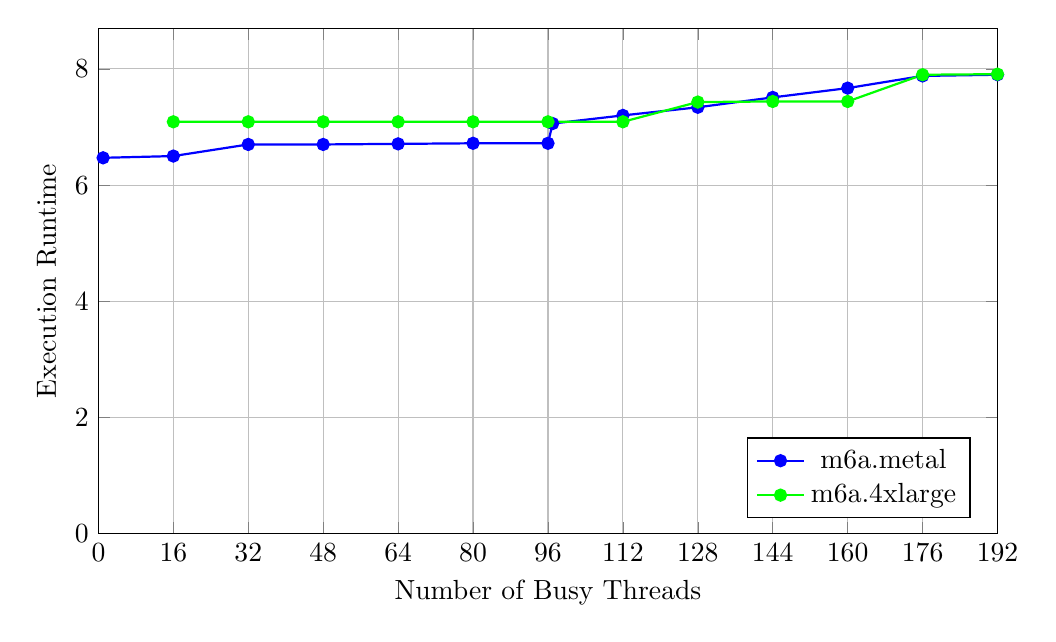
\begin{tikzpicture}
\begin{axis}[
    width=13cm,
    height=8cm,
    ylabel={Execution Runtime},
    xlabel={Number of Busy Threads},
    grid=major,
    ymin=0,
    xmin=0, 
    xmax=192,
    xtick distance= 16,
    legend pos=south east
]

\addlegendentry{m6a.metal}
\addplot[
    color=blue,
    mark= *,
    thick,
] coordinates {
(1, 6.47)
(16, 6.50)
(32, 6.70)
(48, 6.70)
(64, 6.71)
(80, 6.72)
(96, 6.72)
(97, 7.06)
(112, 7.20)
(128, 7.34)
(144, 7.51)
(160, 7.67)
(176, 7.88)
(192, 7.9)
 };

\addlegendentry{m6a.4xlarge}
\addplot[
    color=green,
    mark= *,
    thick,
] coordinates {
(16, 7.09)
(32, 7.09)
(48, 7.09)
(64, 7.09)
(80, 7.09)
(96, 7.09)
(112, 7.09)
(128, 7.43)
(144, 7.44)
(160, 7.44)
(176, 7.90)
(192, 7.91)
 };

\end{axis}
\end{tikzpicture}
\caption{Performance of the test node (while incrementally adding busy neighbors) in comparison to running the threads natively on m6a.metal}
\label{fig::m6a_metal_vs_VMs}
\end{figure}
\noindent
The overall performance degradation for the metal instance is equal to 23.5\%. 
For the first 96 threads, we observe a performance 
degradation of 3.9\%. When adding the 97th thread ($n/2 + 1$), we witness an additional 
degradation of 5.2\%, which is less significant than the degradation we saw at the same level for 
m5 and the m6i dedicated hosts (respectively 25\% and 20\%). 
We observe that the majority of the degradation occurs in the second half of adding the busy threads, 
i.e., from thread 97 to 192. During this phase, the degradation increases almost steadily 
from 9\% to 23\%. The degradation on the second half was also present on the m5 and m6i host 
with respectively 8.63\% and 7\%. 
The first m5.4xlarge (test node) had an initial runtime 9.3\% worse than running \textit{cpu\_burn} with 
16 threads on the m6a.metal instance, which implies the same mapping of the vCPUs across the physical 
cores as discussed previously. \\ 
We have now established that the witnessed degradation in the different families is not caused by 
physical core co-location, as the vCPUs of each VM are isolated. It is also unlikely that it is caused 
by virtualization overhead, as the performance of the metal instance and the VM converge toward
the same value at full capacity. In the following part, we investigate the role of frequency scaling 
in these performance losses (H3). 